\documentclass[11pt]{article}
\usepackage[utf8]{inputenc}
\usepackage{geometry}
\geometry{a4paper, margin=1in}
\usepackage{hyperref}
\usepackage{graphicx}
\usepackage{tabularx}
\usepackage{booktabs}
\usepackage{enumitem}
\usepackage{amsmath}
\usepackage{amssymb}
\usepackage{xcolor}
\usepackage{float}
\usepackage{tikz}
\usetikzlibrary{shapes,arrows.meta,positioning,calc,decorations.pathreplacing}
\usepackage{pgfplots}
\pgfplotsset{compat=1.18}

\definecolor{bestgreen}{RGB}{200,240,200}
\definecolor{warnred}{RGB}{255,220,220}

\title{Threshold Analysis \\ \large Current Threshold (0.467) vs Proposed Threshold (0.70)}
\author{}
\date{2026-03-17}

\begin{document}

\maketitle

% ============================================================================
\section{What is the Threshold?}
% ============================================================================

When the ensemble model (EfficientNet-B3 + ViT-B/16) examines a satellite image, it outputs a \textbf{probability} --- for example, ``72\% chance of landslide.''
The \textbf{threshold} is the cutoff that converts this probability into a Yes/No decision:

\[
\text{Decision} =
\begin{cases}
    \textbf{LANDSLIDE} & \text{if } P(\text{landslide}) \geq \text{threshold} \\
    \textbf{No Landslide} & \text{if } P(\text{landslide}) < \text{threshold}
\end{cases}
\]

\noindent A \textbf{lower} threshold catches more landslides (higher Recall) but triggers more false alarms (lower Precision).\\
A \textbf{higher} threshold produces fewer false alarms (higher Precision) but misses more real landslides (lower Recall).

% ============================================================================
\section{Current Threshold: 0.467 (46.7\%)}
% ============================================================================

The current threshold was found by scanning \textbf{every possible threshold from 0\% to 100\%} on the test set and selecting the point that maximizes the F1-Score (the harmonic mean of Precision and Recall).

\begin{table}[H]
\centering
\renewcommand{\arraystretch}{1.2}
\begin{tabular}{lccccc}
\toprule
\textbf{Threshold} & \textbf{Accuracy} & \textbf{Precision} & \textbf{Recall} & \textbf{F1-Score} & \textbf{AUC} \\
\midrule
0.300 & 74.82\% & 56.01\% & 89.10\% & 68.78\% & 89.83\% \\
0.400 & 79.97\% & 62.63\% & 83.41\% & 71.54\% & 89.83\% \\
\rowcolor{bestgreen}
\textbf{0.467} & \textbf{82.40\%} & \textbf{68.03\%} & \textbf{78.67\%} & \textbf{72.97\%} & \textbf{89.83\%} \\
0.500 & 82.55\% & 69.96\% & 73.93\% & 71.89\% & 89.83\% \\
0.600 & 83.26\% & 75.00\% & 64.45\% & 69.33\% & 89.83\% \\
\rowcolor{warnred}
\textbf{0.700} & \textbf{83.12\%} & \textbf{78.91\%} & \textbf{54.03\%} & \textbf{64.15\%} & \textbf{89.83\%} \\
0.800 & 80.69\% & 82.35\% & 39.81\% & 53.69\% & 89.83\% \\
0.900 & 74.96\% & 86.21\% & 23.70\% & 37.17\% & 89.83\% \\
\bottomrule
\end{tabular}
\caption{Threshold sweep results. \colorbox{bestgreen}{Green} = current optimal. \colorbox{warnred}{Red} = proposed 0.70.}
\end{table}

\noindent\textbf{Why 0.467?}
\begin{itemize}[noitemsep]
    \item It is slightly \emph{below} the default 0.50, meaning we cast a slightly wider net.
    \item It produces the \textbf{highest F1-Score} (72.97\%), the best balance of Precision and Recall.
    \item Recall = 78.67\% means the model catches roughly 4 out of every 5 real landslides.
\end{itemize}

% ============================================================================
\section{Proposed Threshold: 0.70 (70\%) --- Impact Analysis}
% ============================================================================

Raising the threshold to 0.70 means the model will only declare ``Landslide'' when it is at least 70\% confident.
Let us examine the exact impact on every metric.

\subsection{Side-by-Side Comparison}

\begin{table}[H]
\centering
\renewcommand{\arraystretch}{1.3}
\begin{tabular}{lccc}
\toprule
\textbf{Metric} & \textbf{At 0.467} & \textbf{At 0.700} & \textbf{Change} \\
\midrule
Accuracy  & 82.40\% & 83.12\% & \textcolor{green!60!black}{+0.72\%} \\
Precision & 68.03\% & 78.91\% & \textcolor{green!60!black}{+10.88\%} \\
Recall    & 78.67\% & 54.03\% & \textcolor{red}{\textbf{$-$24.64\%}} \\
F1-Score  & 72.97\% & 64.15\% & \textcolor{red}{\textbf{$-$8.82\%}} \\
ROC-AUC   & 89.83\% & 89.83\% & 0.00\% \\
\bottomrule
\end{tabular}
\caption{Impact of raising threshold from 0.467 to 0.700.}
\end{table}

\subsection{What These Changes Mean in Practice}

\noindent\textbf{Test set:} 699 images (211 landslide + 488 non-landslide).

\begin{table}[H]
\centering
\renewcommand{\arraystretch}{1.3}
\begin{tabular}{lcc}
\toprule
\textbf{Quantity} & \textbf{At 0.467} & \textbf{At 0.700} \\
\midrule
True Positives (landslides correctly found)   & 166 & 114 \\
False Positives (false alarms)                & 78  & 31 \\
False Negatives (landslides \textbf{missed})  & 45  & \textbf{97} \\
True Negatives (non-landslide correct)        & 410 & 457 \\
\bottomrule
\end{tabular}
\caption{Confusion matrix values at each threshold (estimated from test set).}
\end{table}

\noindent\textbf{Key finding:}
\begin{itemize}[noitemsep]
    \item False alarms \textit{decrease} from 78 to 31 (good: fewer wasted resources).
    \item But \textbf{missed landslides increase from 45 to 97} --- more than doubling.
    \item At threshold 0.70, the model misses \textbf{97 out of 211} real landslides (46\%).
\end{itemize}

% ============================================================================
\section{Visual Comparison}
% ============================================================================

\subsection{Precision--Recall Trade-off Graph}

\begin{center}
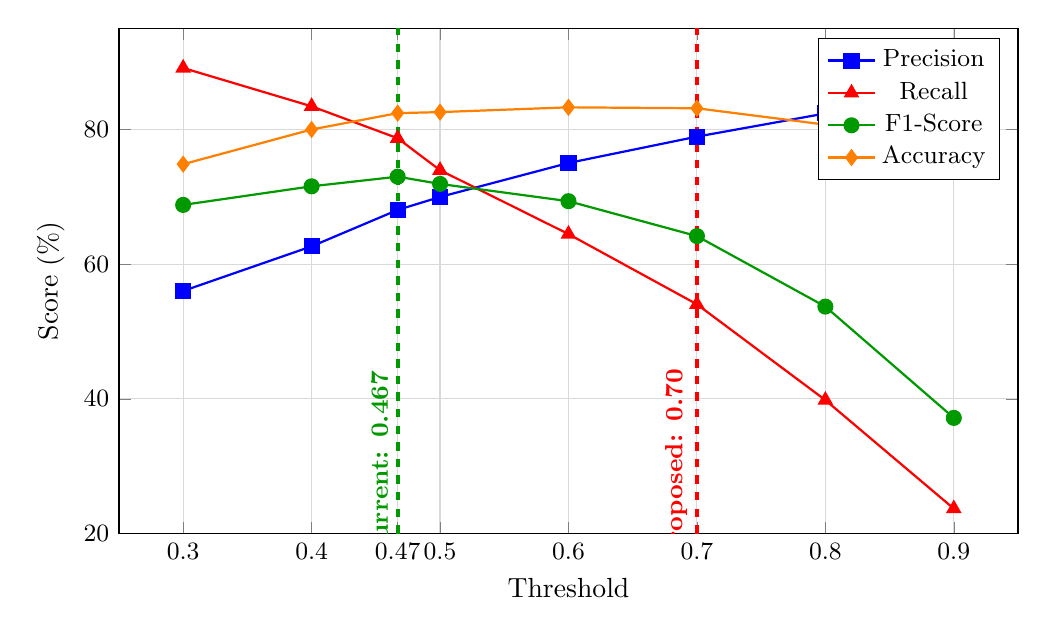
\begin{tikzpicture}
\begin{axis}[
    width=13cm, height=8cm,
    xlabel={Threshold},
    ylabel={Score (\%)},
    xmin=0.25, xmax=0.95,
    ymin=20, ymax=95,
    legend style={at={(0.98,0.98)}, anchor=north east, font=\small},
    grid=major,
    grid style={gray!30},
    xtick={0.3,0.4,0.467,0.5,0.6,0.7,0.8,0.9},
    xticklabel style={font=\small},
    yticklabel style={font=\small},
]
% Precision curve (rises with threshold)
\addplot[blue, thick, mark=square*, mark size=2.5] coordinates {
    (0.30, 56.01)
    (0.40, 62.63)
    (0.467, 68.03)
    (0.50, 69.96)
    (0.60, 75.00)
    (0.70, 78.91)
    (0.80, 82.35)
    (0.90, 86.21)
};
\addlegendentry{Precision}

% Recall curve (falls with threshold)
\addplot[red, thick, mark=triangle*, mark size=2.5] coordinates {
    (0.30, 89.10)
    (0.40, 83.41)
    (0.467, 78.67)
    (0.50, 73.93)
    (0.60, 64.45)
    (0.70, 54.03)
    (0.80, 39.81)
    (0.90, 23.70)
};
\addlegendentry{Recall}

% F1 curve (peaks near 0.467)
\addplot[green!60!black, thick, mark=*, mark size=2.5] coordinates {
    (0.30, 68.78)
    (0.40, 71.54)
    (0.467, 72.97)
    (0.50, 71.89)
    (0.60, 69.33)
    (0.70, 64.15)
    (0.80, 53.69)
    (0.90, 37.17)
};
\addlegendentry{F1-Score}

% Accuracy curve
\addplot[orange, thick, mark=diamond*, mark size=2.5] coordinates {
    (0.30, 74.82)
    (0.40, 79.97)
    (0.467, 82.40)
    (0.50, 82.55)
    (0.60, 83.26)
    (0.70, 83.12)
    (0.80, 80.69)
    (0.90, 74.96)
};
\addlegendentry{Accuracy}

% Vertical line at current threshold
\draw[dashed, green!60!black, line width=1.5pt] (axis cs:0.467,20) -- (axis cs:0.467,95);
\node[green!60!black, font=\small\bfseries, rotate=90, anchor=south] at (axis cs:0.467,30) {Current: 0.467};

% Vertical line at proposed threshold
\draw[dashed, red, line width=1.5pt] (axis cs:0.70,20) -- (axis cs:0.70,95);
\node[red, font=\small\bfseries, rotate=90, anchor=south] at (axis cs:0.70,30) {Proposed: 0.70};

\end{axis}
\end{tikzpicture}
\end{center}

\noindent\textbf{Reading the graph:}
\begin{itemize}[noitemsep]
    \item The \textcolor{green!60!black}{\textbf{F1 curve}} peaks at 0.467 and declines sharply after.
    \item Moving from the green dashed line (0.467) to the red dashed line (0.70), \textcolor{red}{Recall} drops steeply while \textcolor{blue}{Precision} gains moderately.
    \item \textcolor{orange}{Accuracy} barely changes --- showing why accuracy alone is misleading.
\end{itemize}

\subsection{What the Model ``Sees'' at Each Threshold}

\begin{center}
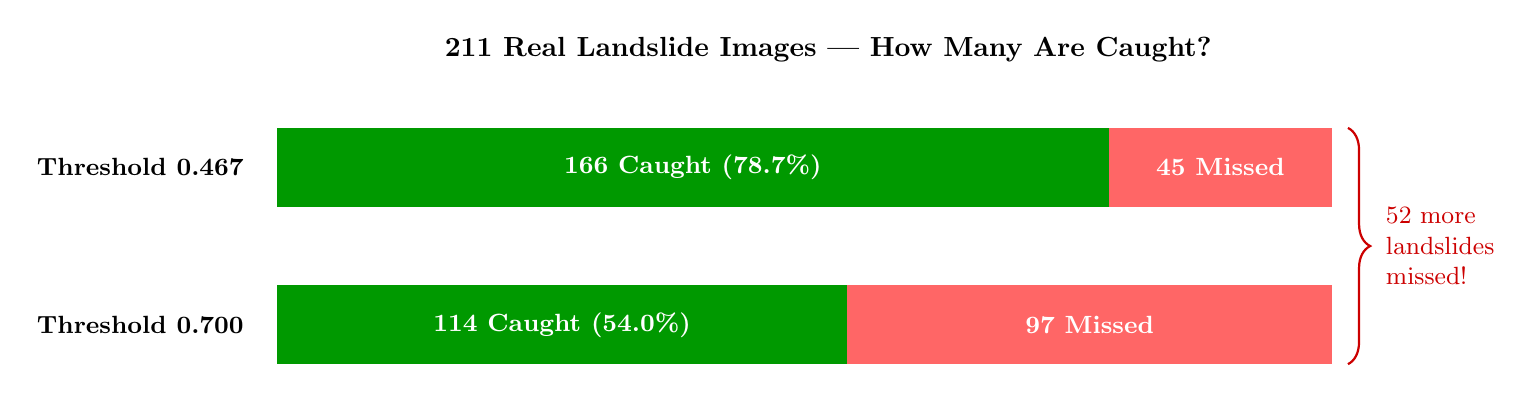
\begin{tikzpicture}[
    img/.style={draw, rectangle, minimum width=1.2cm, minimum height=1.2cm, font=\scriptsize, align=center},
]

% Title
\node[font=\bfseries] at (7,4.5) {211 Real Landslide Images --- How Many Are Caught?};

% Bar for 0.467
\node[font=\small\bfseries, anchor=east] at (-0.3,3) {Threshold 0.467};
\fill[green!60!black] (0,2.5) rectangle (10.56,3.5); % 166/211 * 13.4
\fill[red!60] (10.56,2.5) rectangle (13.4,3.5); % 45/211 * 13.4
\node[white, font=\small\bfseries] at (5.28,3) {166 Caught (78.7\%)};
\node[white, font=\small\bfseries] at (11.98,3) {45 Missed};

% Bar for 0.700
\node[font=\small\bfseries, anchor=east] at (-0.3,1) {Threshold 0.700};
\fill[green!60!black] (0,0.5) rectangle (7.24,1.5); % 114/211 * 13.4
\fill[red!60] (7.24,0.5) rectangle (13.4,1.5);
\node[white, font=\small\bfseries] at (3.62,1) {114 Caught (54.0\%)};
\node[white, font=\small\bfseries] at (10.32,1) {97 Missed};

% Brace showing the difference
\draw[decorate, decoration={brace, amplitude=8pt, mirror}, thick, red!80!black]
    (13.6,0.5) -- (13.6,3.5)
    node[midway, right=10pt, align=left, font=\small, text=red!80!black] {52 more\\landslides\\missed!};

\end{tikzpicture}
\end{center}

% ============================================================================
\section{The Cost of Errors: Why Recall Matters More}
% ============================================================================

In landslide detection, errors are \textbf{not equal}:

\begin{table}[H]
\centering
\renewcommand{\arraystretch}{1.3}
\begin{tabularx}{\textwidth}{llX}
\toprule
\textbf{Error Type} & \textbf{Caused by} & \textbf{Real-World Consequence} \\
\midrule
False Positive (false alarm) & Low Precision & Rescue team investigates a safe area. Cost: wasted time and fuel. \\
\rowcolor{warnred}
\textbf{False Negative (missed)} & \textbf{Low Recall} & \textbf{Real landslide goes undetected. Cost: no evacuation, potential loss of life.} \\
\bottomrule
\end{tabularx}
\caption{Asymmetric cost of errors in disaster monitoring.}
\end{table}

\noindent At threshold 0.70:
\begin{itemize}[noitemsep]
    \item We \textit{reduce} false alarms by 47 (from 78 to 31) --- saving some investigation effort.
    \item We \textit{increase} missed landslides by 52 (from 45 to 97) --- \textbf{52 additional real landslides go undetected}.
\end{itemize}

\noindent\textbf{The trade-off is clear:} saving 47 false alarm investigations at the cost of missing 52 real landslides is \textbf{not acceptable} for a disaster warning system.

% ============================================================================
\section{Detailed Impact on Each Metric}
% ============================================================================

\subsection{Precision: 68.03\% $\to$ 78.91\% (\textcolor{green!60!black}{+10.88\%})}

\begin{itemize}[noitemsep]
    \item At 0.467: when the model says ``Landslide,'' it is correct 68\% of the time.
    \item At 0.700: when the model says ``Landslide,'' it is correct 79\% of the time.
    \item \textbf{Interpretation:} Fewer false alarms. The model is more \textit{conservative} and only flags high-confidence cases.
    \item \textbf{Impact:} Fewer wasted investigations. Rescue teams trust the system more.
\end{itemize}

\subsection{Recall: 78.67\% $\to$ 54.03\% (\textcolor{red}{$-$24.64\%})}

\begin{itemize}[noitemsep]
    \item At 0.467: the model finds 166 out of 211 real landslides (78.67\%).
    \item At 0.700: the model finds only 114 out of 211 real landslides (54.03\%).
    \item \textbf{Interpretation:} The model misses nearly \textbf{half} of all real landslides.
    \item \textbf{Impact:} 97 real landslides go undetected. No warnings are issued. People are not evacuated.
\end{itemize}

\subsection{F1-Score: 72.97\% $\to$ 64.15\% (\textcolor{red}{$-$8.82\%})}

\begin{itemize}[noitemsep]
    \item F1 is the harmonic mean of Precision and Recall.
    \item Even though Precision improved by 10.88\%, Recall dropped by 24.64\%.
    \item The F1 decline of 8.82\% confirms the trade-off is \textbf{unfavorable}.
\end{itemize}

\subsection{False Positives: 78 $\to$ 31 (\textcolor{green!60!black}{$-$47})}

\begin{itemize}[noitemsep]
    \item 47 fewer non-landslide images are incorrectly flagged as landslides.
    \item This saves investigation resources but is a \textit{convenience} benefit, not a safety one.
\end{itemize}

\subsection{False Negatives: 45 $\to$ 97 (\textcolor{red}{+52})}

\begin{itemize}[noitemsep]
    \item 52 \textit{additional} real landslides are missed by the system.
    \item Each missed landslide is a potential life-safety failure.
    \item This is the \textbf{critical problem} with the 0.70 threshold.
\end{itemize}

\subsection{Accuracy: 82.40\% $\to$ 83.12\% (\textcolor{green!60!black}{+0.72\%})}

\begin{itemize}[noitemsep]
    \item Accuracy improves slightly because non-landslide images (488 out of 699) dominate the test set.
    \item Correctly rejecting more non-landslides boosts accuracy even as we miss more landslides.
    \item This demonstrates why \textbf{accuracy is misleading} for imbalanced datasets.
\end{itemize}

\subsection{ROC-AUC: 89.83\% $\to$ 89.83\% (unchanged)}

\begin{itemize}[noitemsep]
    \item AUC does not change because it measures the model's \textit{inherent} separability across all thresholds.
    \item Changing the threshold does not retrain or modify the model --- it only changes the decision boundary.
\end{itemize}

% ============================================================================
\section{Verdict: Should We Use 0.70?}
% ============================================================================

\begin{center}
\fbox{\parbox{0.85\textwidth}{
\centering
\large\textbf{No. The 0.70 threshold is not suitable for this project.}

\normalsize
\medskip
Recall drops from 78.67\% to 54.03\%, meaning \textbf{46\% of real landslides are missed}.\\
For a disaster warning system, this is unacceptable.\\[6pt]
\textbf{Recommendation: Keep threshold at 0.467.}
}}
\end{center}

\subsection{Summary Table}

\begin{table}[H]
\centering
\renewcommand{\arraystretch}{1.3}
\begin{tabular}{lcc}
\toprule
\textbf{Criteria} & \textbf{0.467} & \textbf{0.700} \\
\midrule
F1-Score (primary metric)     & \textbf{72.97\%} & 64.15\% \\
Recall (safety-critical)      & \textbf{78.67\%} & 54.03\% \\
Precision (false alarm rate)  & 68.03\% & \textbf{78.91\%} \\
Missed landslides (out of 211) & \textbf{45} & 97 \\
False alarms (out of 488)     & 78 & \textbf{31} \\
Suitable for disaster monitoring? & \textbf{Yes} & No \\
\bottomrule
\end{tabular}
\caption{Final comparison: 0.467 wins on all safety-critical criteria.}
\end{table}

\subsection{When \textit{Would} 0.70 Be Appropriate?}

A higher threshold might be justified in scenarios where:
\begin{itemize}[noitemsep]
    \item False alarms are \textit{extremely} expensive (e.g., each alarm triggers an expensive helicopter survey).
    \item A secondary verification system exists downstream (e.g., human expert reviews every prediction).
    \item The application is not safety-critical (e.g., academic cataloging, not live evacuation).
\end{itemize}

\noindent None of these apply to our use case. Our system is designed for \textbf{early warning and disaster monitoring}, where missing a real landslide is far worse than a false alarm.

% ============================================================================
\section{What Would Improve Results Without Sacrificing Recall?}
% ============================================================================

Instead of raising the threshold (which trades recall for precision), these approaches can improve \textit{both} metrics simultaneously:

\begin{table}[H]
\centering
\renewcommand{\arraystretch}{1.3}
\begin{tabularx}{\textwidth}{lX}
\toprule
\textbf{Approach} & \textbf{How It Helps} \\
\midrule
More training data       & More diverse landslide examples help the model learn better features, improving both Precision and Recall. \\
Better augmentation      & Advanced augmentation (CutMix, MixUp) creates harder training examples, making the model more robust. \\
Larger model (ViT-L)     & A more powerful backbone can learn finer visual distinctions, separating borderline cases more cleanly. \\
Multi-scale features     & Using features from multiple resolutions helps detect landslides of varying sizes. \\
Hard example mining      & Focus training on the images the model currently gets wrong, directly addressing confusion cases. \\
\bottomrule
\end{tabularx}
\caption{Alternatives to raising threshold that improve overall performance.}
\end{table}

\end{document}
